\label{ch:analysis}

With the purpose of providing a deeper understanding on how some of the most relevant datasets regarding fall detection were collected, an analysis was performed in order to identify common \textbf{patterns}, the \textbf{technologies} employed and the \textbf{results obtained}. Afterwards, the previously mentioned \textbf{Electrodermal Activity} and its potential implications in the context of fall detection were both investigated.

\section{Typical biometric data employed in fall detection}\label{sec:hardware}

The consequences of falling may be observed through a series of data that addresses aspects related to physical, physiological and environmental variables. Some of the repercussions that a hard fall may cause are:

\begin{itemize}
    \item A fast shift of the gravitational acceleration values
    \item A change of the altitude above ground level
    \item Feelings of fear and obfuscation (especially for elderly people in severe cases)
    \item A decrease of the body temperature (in cases in which the individual remains prone on the ground for extended periods of time)
\end{itemize}

The following section introduces some of the most commonly used instruments to retrieve data that may be functional to fall detection systems.

\subsection{Accelerometer}\label{subsec:accelerometer}

The accelerometer provides a measure of the \textbf{acceleration} in relation to an entity in its coordinate system. Once calibrated, the obtained value measures 9.81 $m/s^2$ at rest (which corresponds to the gravity acceleration) and drops at 0 $m/s^2$ during a \textbf{free fall}.

Furthermore, modern accelerometer are commonly implemented as \emph{micro-electro-mechanical-systems} and their dimensions have packaged sizes of only 2 x 2 x 1 \textit{mm}. This makes them particularly suitable for \textbf{wearable devices} and \textbf{embedded systems}.

Since a 3-axis accelerometer provides a separate trace for the $x$, $y$ and $z$ axis, a \textbf{magnitude vector} can be computed in order to represent the measurement as a scalar value. The formula involves the calculation of the norm of the coordinate vector and is generally computed in real-time on embedded systems in order to provide a value for classification purposes.

\newcommand\norm[1]{\left\lVert#1\right\rVert}

\begin{figure}[h]
    \begin{equation}
    \norm{a}_2 = \sqrt{a_{x}^2 + a_{y}^2 + a_{z}^2}
    \end{equation}
    \caption{Magnitude Vector formula}
    \label{fig:magnitude}
\end{figure}

\subsection{9-Axis IMUs}\label{subsec:imus}

The \textbf{inertial motion sensor} units (commonly referred as IMUs) provide a combination of three sensors:

\begin{itemize}
    \item A 3-axis accelerometer
    \item A 3-axis gyroscope 
    \item A 3-axis magnetometer 
\end{itemize}

While the accelerometer and gyroscope signals provide measures to describe the \emph{rotation} and the \emph{acceleration} around each axis, a magnetometer is employed in order to sense the surrounding \emph{magnetic field} and correct small drifts over long lasting periods of time. 

The combination of the latter sources provides a criteria to compute the \textbf{complete orientation in space} and offers remarkable advantages in order to improve accuracy in motion tracking and fall detection systems.

\subsection{Barometric Altimeter}\label{subsec:altimeter}

The barometric altimeter determines changes in elevation by employing a pressure sensor. Compared to the changes in the atmospheric pressure, in fact, the altitude variation result inversely proportional \cite{mems-altimeter}.

Although barometric altimeters are involved in a multitude of usages the data collected may provide useful information in the context of fall detection systems. The altitude level, when combined with the data retrieved from a 9-Axis IMU or an accelerometer, may confirm that a fall event just happened with higher levels of accuracy.

Several instruments for motion tracking include both a 9-Axis inertial measurement unit and a barometric altimeter. For that, they are commonly referred as \textbf{10-Axis IMUs}.

\subsection{Biometric Sensors}\label{subsec:biometric-sensors}

Another branch of information which has been widely regarded lately is related to biometric sensors. These include a variety of instruments to collect biometric signals by using appropriate hardware, such as \textbf{electrodes}, \textbf{skin contact technologies} and others.

Besides some units require the usage of specific hardware, other sensors (such as the ECG, EEG, Temperature, EDA and others) have already been implemented in several commercial wearable devices and provide accurate data that can later be involved in the computation of several biometric descriptors. 

In the context of fall detection systems, a synchronized retrieval of both biometric and motion related data may significantly improve the accuracy of classification models.

\section{Multimodal datasets for fall detection systems}\label{sec:datasets}

Despite the fact that various falls datasets have been made available throughout the years, two of them were selected for the purpose of this analysis as a consequence of their relevance in the research environment.

\subsection{UMAFall - A Multisensor Dataset for the Research on Automatic Fall Detection}\label{subsec:umafall}

The \textbf{UMAFall} dataset gained considerable interest since its publication (happened in 2017). The primary difference from other datasets was, in fact, related to the way Casilari \textit{et al., 2018}~\cite{umafall} approached the data collection stage, which involved the usage of multiple units of the same sensor. 

Basing on the conclusions drawn by previous publications, UMAFall was designed in order to provide a public dataset to study the importance of sensor units placement for the effectiveness of fall detection algorithms \cite{umafall}. The traces collected provide measurements of the mobility during daily life activities and falls, obtained by \textbf{five sensing nodes} placed on different positions of the body of several individuals.

\subsubsection{Technologies Involved}\label{subsubsec:umafall-technologies}

The data gathering architecture was implemented as a \textbf{Bluetooth Low Energy} (BLE) piconet composed of:

\begin{itemize}
    \item Four wearable sensors located in four different positions of the body, acting as \textbf{slave nodes}
    \item An Android smartphone, acting as the \textbf{master node}
\end{itemize}

The nodes were implemented through multiple \textbf{SimpleLink SensorTag} units. These consist of IoT devices powered by a CC2650 ARM microcontroller that integrates: 

\begin{itemize}
    \item a 2.4 GHz transceiver
    \item 10 embedded sensors, including an MPU-9250 multichip module
\end{itemize}

The latter made possible the retrieval of motion related data, combining the values registered by a 3-axis gyroscope, a 3-axis accelerometer and a 3-axis magnetometer, which were regularly sent to the master unit and later saved in a CSV file. However, the usage of the Bluetooth protocol has demanded low resolutions in order to avoid saturating the communication channel. Therefore, the \textbf{sample rate} was set to 20 Hz for each unit.

\subsubsection{Activities Performed}\label{subsubsec:umafall-activities}

The four sensors were placed on locations typically reported in literature, such as the ankle, waist, chest and right wrist. Furthermore, the participants consisted of seventeen individuals divided in ten males and seven females aged between 18 and 55 years old.

Because of the practical sensor architecture based on wearable devices, data could be retrieved in a domestic environment and included the activities reported in Table \ref{toc:umafall}

\begin{table}[H]
\centering
\begin{tabular}{ll}
    \hline
    Activity                & Category \\
    \hline
    Body bending            & Daily Activities \\
    Climbing stairs down    & Daily Activities \\
    Hopping                 & Daily Activities \\
    Light jogging           & Daily Activities \\
    Lying down              & Daily Activities \\
    Sitting down            & Daily Activities \\
    Walking                 & Daily Activities \\
    Forward fall            & Fall \\
    Later fall              & Fall \\
    Backwards fall          & Fall \\
    \hline
\end{tabular}
\caption{Activities evaluated in UMAFall}
\label{toc:umafall}
\end{table}

\subsubsection{Results Obtained}\label{subsubsec:umafall-results}

Casilari \textit{et al., 2018}~\cite{umafall} provided a dataset including 531 CSV files of which 322 were reporting daily activities data and 209 were reporting falls related data, each one of 15-seconds duration. An initial analysis was performed in order to describe the variation of the \textbf{Signal Magnitude Vector} for each dataset.

Lastly, the results obtained determined substantial difficulties in distinguishing falls from moderate activities using threshold based techniques. An approach based on the fusion of multiple sensor data and the usage of Machine Learning advances in order to reduce the number of \textbf{false positives} obtained was, lastly, proposed by the authors, but not implemented.

\subsection{UP-Fall Detection Dataset: A Multimodal Approach}\label{sec:upfall}

The \textbf{UP-Fall} dataset was presented in 2019 in order to collect fall-related information according to three major modalities:

\begin{itemize}
    \item \textbf{Wearable sensors}
    \item \textbf{Ambient sensors}
    \item \textbf{Vision devices}
\end{itemize}

The aim of the study was providing a considerable amount of data collected from heterogeneous sources in order to address the lack of publicly available measurements for the evaluation of fall detection systems \cite{upfall}.

\subsubsection{Technologies Involved}\label{subsubsec:upfall-technologies}

The hardware involved consisted of: 

\begin{itemize}
\item Five \textbf{Mbientlab MetaSensor} wearables located in different points of the body and collecting data from: 
    \begin{itemize}
        \item A 3-axis accelerometer
        \item A 3-axis gyroscope
        \item An ambient light sensor
    \end{itemize}
\item A \textbf{NeuroSky MindWave} electroencephalograph headset measuring the brainwave signal
\item Six \textbf{infrared sensors} forming a grid above the floor of the room
\item Two \textbf{Microsoft LifeCam Cinema} cameras providing a frontal and a lateral view of the individual 
\end{itemize}

The data gathering architecture was implemented through the usage of two computers and three Raspberry PI V3 in order to collect the information from all the sensors and later save it in the form of multiple CSV files.

In this case a sample rate of \~ 18.4 Hz was configured in order to accommodate the requirements of all the units involved.

\subsubsection{Activities Performed}\label{subsubsec:upfall-activities}

The UP-Fall dataset was collected in a \textbf{controlled environment} where 17 young and healthy subjects were required to perform 11 different activities with three attempts each \cite{upfall}.

\begin{table}[H]
\centering
\begin{tabular}{ll}
    \hline
    Activity                          &   Category           \\
    \hline
    Walking                           &   Daily Activities   \\
    Standing                          &   Daily Activities   \\
    Sitting                           &   Daily Activities   \\
    Picking up an Object              &   Daily Activities   \\
    Laying                            &   Daily Activities   \\
    Jumping                           &   Daily Activities   \\
    Falling sitting in empty chair    &   Fall               \\
    Falling sideward                  &   Fall               \\
    Falling backwards                 &   Fall               \\
    Falling forwards using knees      &   Fall               \\
    Falling forwards using hands      &   Fall               \\
    \hline
\end{tabular}
\caption{Activities evaluated in UP-Fall}
\label{toc:umafall2}
\end{table}

The raw gathered data was later divided in different time windows and, for each one of them, a \textbf{feature extraction and selection} process was performed. The processed information was, then, used to evaluate the performance of four classification models: 

\begin{itemize}
    \item Random Forest
    \item Support Vector Machines
    \item Multi-Layer Perceptron
    \item \textit{k}-Nearest Neighbors
\end{itemize}

The performances of the latter were evaluated through the metrics of \textit{accuracy}, \textit{precision}, \textit{sensitivity}, \textit{specificity} and $F_1$ - \textit{score}.

A limitation pointed out by the authors \cite{umafall} involves the context of the experimentation: the falls performed were self-initiated and different from real-life falls. These kind of aspects constitute a primary concern for researchers because of the difficulties in addressing them and the inaccuracy they might lead to, as stated in \ref{sec:fallintro}.

\subsubsection{Results Obtained}\label{subsubsec:upfall-results}

The dataset obtained and the following activities of processing and subsequent analysis performed led to observe that the data retrieved from the inertial measurement units of the wearables played a major role in the accuracy of the classification models. The accuracy (depicted by the $F_1$-score) of the IMUs-only based classification reached a value of 70.31\% while classifiers trained with combination of infrared and camera data demonstrated considerably lower performances (between 15\% and 33\%). Lastly, the combination of data collected by wearables, cameras and the EEG sensor obtained the highest $F_1$-score accuracy measure, which corresponded to 70.44\%. 

Additionally, a Convolutional Neural Network was trained in order to improve the classification performance based on video recording data. This reached an $F_1$-\textit{score} of 71.2\%.

In conclusion, in the context of fall detection systems, the analysis performed on the UP-Fall dataset demonstrated that a certain degree of accuracy may be reached by processing data from sources of different nature, even though classifications can be improved by approaching the subject in a multimodal and heterogeneous manner.

\section{Electrodermal Activity}\label{sec:eda-description}

In the whole field of bio-signals, a subject of interest in the recent years has been the so-called \textbf{Electrodermal Activity}, also known as \textbf{Skin Conductance} or \textbf{Galvanic Skin Response}.

The latter describes the continuous variations of the electrical conductivity of the skin (which is also referred as Skin Conductance or SC) and has been depicted as the main criteria to investigate the psychophysiological states of an individual since the beginning of the 20th century.

\subsection{EDA signals and correlation with psychophysiological stress detection}\label{subsec:eda-signals}

As stated in section \ref{sec:edaintro}, the Electrodermal Activity provides a non-invasive technique to analyze the activity of the \textbf{autonomic nervous system} (ANS) by measuring the resistance opposed by the skin to the electrical current, which varies according to the \textbf{sweat glands} activity.

Perspiration is, in fact, governed by the sympathetic nervous system \cite{bartholomew} through the postganglionic sudomotor fibers, in connection with the external stimulations received. On these principles, a situation of emotional distress that induces an excitement of the ANS activity would also cause changes in sweat secretion. The measuring of the latter may, then, provide a qualitative indicator related to the \textbf{emotional response} of a subject \cite{carlson}.

\begin{figure}[h]
    \centering
    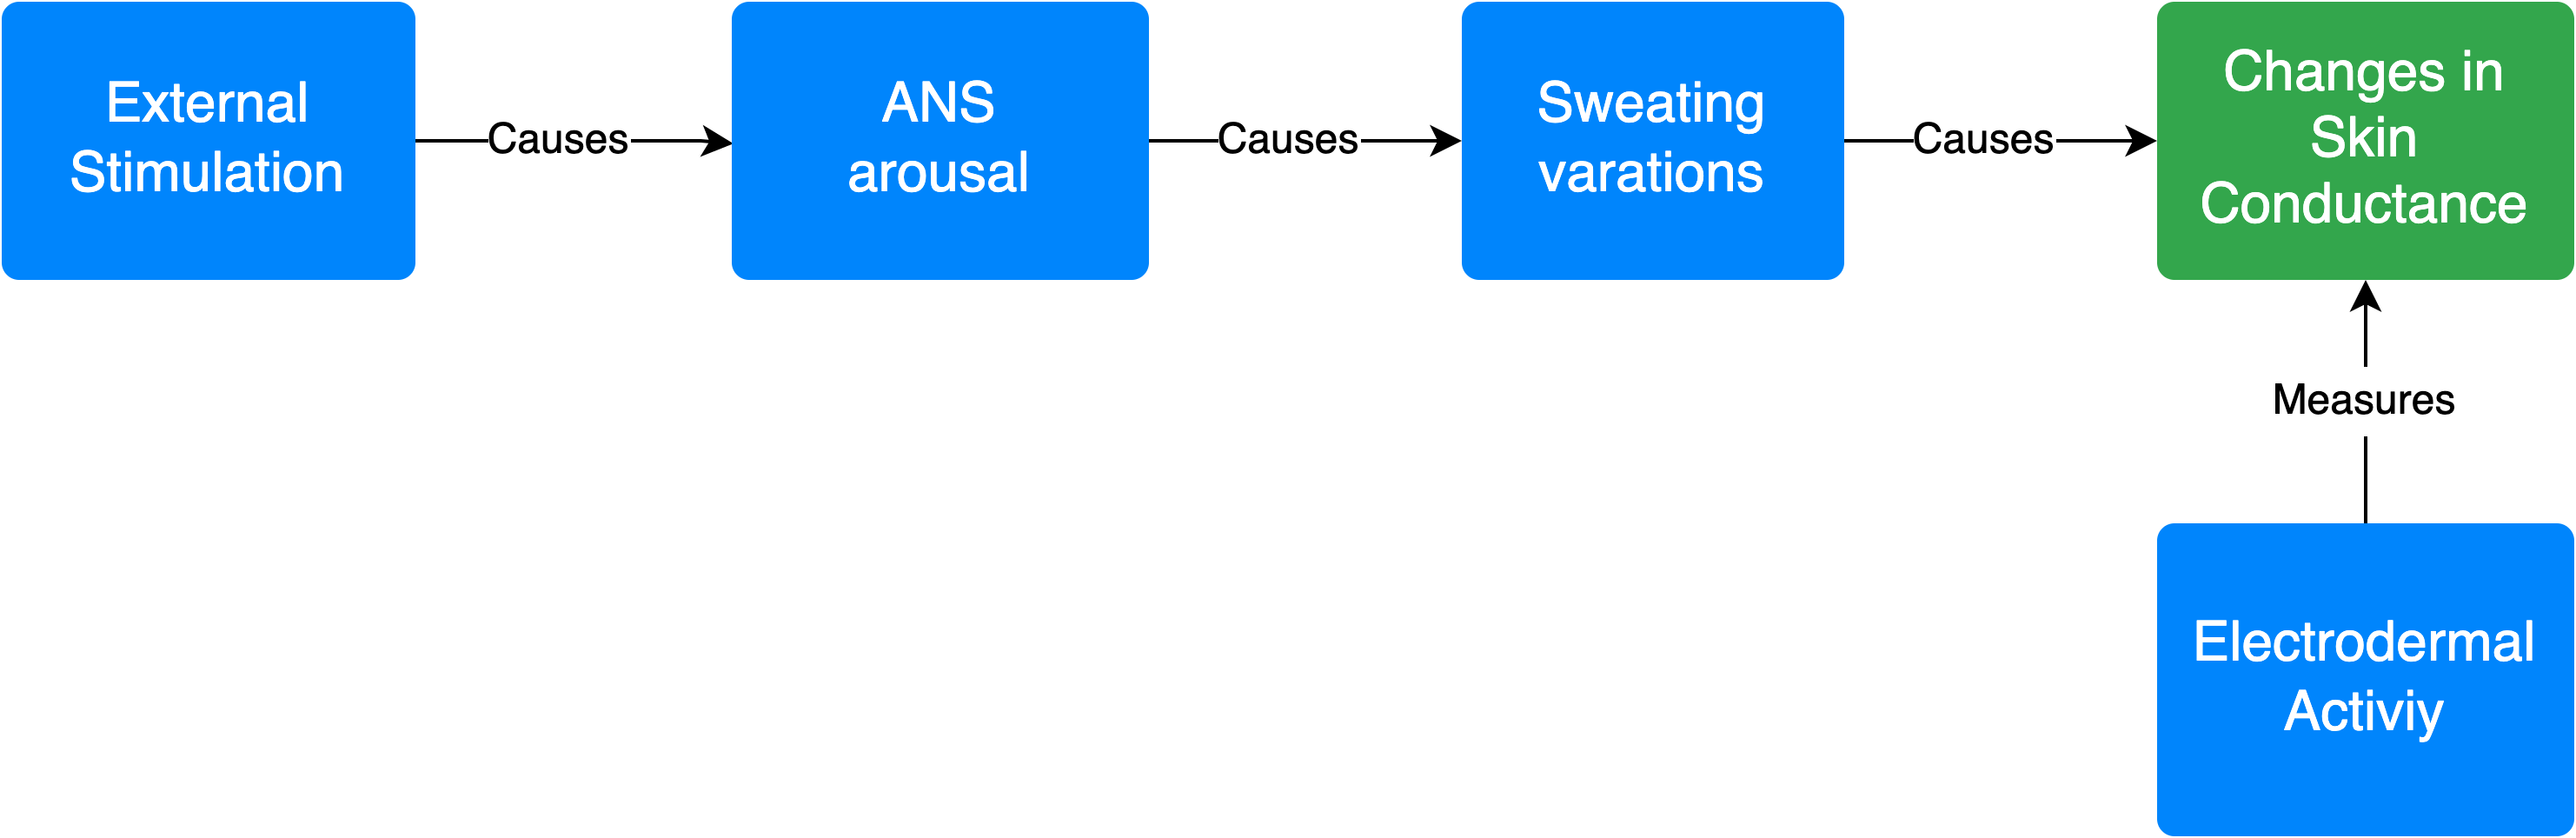
\includegraphics[width=\textwidth]{./images/eda-cause-effect.drawio.png}
    \caption{Correlation between Electrodermal Activity and the Autonomic Nervous System}
    \label{fig:eda-ans}
\end{figure}

\subsection{Measurement}\label{subsec:eda-measurement}

% https://www.birmingham.ac.uk/Documents/college-les/psych/saal/guide-electrodermal-activity.pdf

In order to detect Electrodermal Activity on and individual's skin, two different approaches may be employed:

\begin{itemize}
    \item Exosomatic Methodology
    \item Endosomatic Methodology
\end{itemize}

The first one tends to be the most commonly used and implies the application of a direct or alternating current directly on the skin. The second one, instead, does not involve the usage of any external current.

% https://www.tobiipro.com/learn-and-support/learn/GSR-essentials/how-does-a-gsr-sensor-work/
The implementation of the exosomatic methodology requires the usage of \textbf{two electrodes} through which a voltage of direct current of 0.5 VDC is trasmitted. After being applied to the skin, the current flow through the electrodes is measured by applying the \textbf{Ohm's Law}, which determines the resistance opposed by the epidermis.

\begin{figure}[h]
    \begin{equation}
    \begin{aligned}
    I = \frac{U}{R} \\
    \\
    R = \frac{U}{I}
    \end{aligned}
    \end{equation}
    \caption{Ohm's Law Formula}
    \label{fig:ohmlaw}
\end{figure}

It is important to place both the electrodes on the palm of the hand, on two adjacent fingers or, otherwise, on the sole of the foot. These areas have been, in fact, identified as the most prominent in terms of perspiration. Modern EDA sensors employ electrodes with Ag/AgCl contact points in order to accurately transmit the electrical current \cite{eda-imotions}. Isotonic gel is also generally used to accommodate the signal transmission from the skin and consequently improve its quality.

\begin{figure}[h]
    \centering
    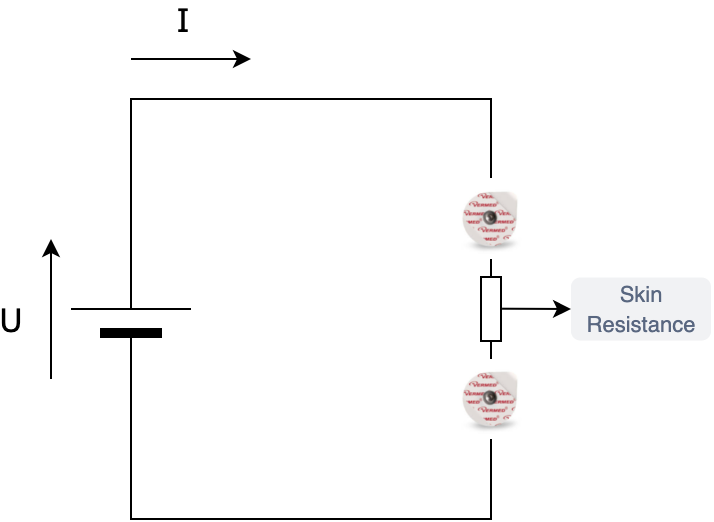
\includegraphics[width=8cm]{./images/skin-resistance.drawio.png}
    \caption{Representation of the EDA measurement principle}
    \label{fig:eda-ans}
\end{figure}

The resistance obtained is expressed in terms of the \textbf{Siemens} ($S$) measuring unit. More specifically, because of the small values obtained, microSiemens ($\mu S$) are normally employed.

\subsection{Sample rates}\label{subsec:eda-signal-properties}

EDA is regarded as a slow measure \cite{eda-guide}. According to the related literature, typical frequency intervals are, in fact:

\begin{itemize}
    \item 0 - 3 Hz \cite{biosignalplux-guide}
    \item 0 - 10 Hz \cite{eda-hci}
    \item 0.0167 - 0.25 Hz \cite{eda-interval-3}
    \item 0.045 - 0.25 Hz \cite{eda-interval-4}
    \item 0.05 - 35 Hz \cite{eda-guide}
\end{itemize}

By applying the \textbf{Nyquist Theorem} \cite{nyquist}, which states that a signal should be sampled at least at two times its highest frequency, it can be inferred that EDA signals must be sampled at 70 Hz or more. In practice, sample rates between 70 Hz and 400 Hz are commonly used according to the requirements of the experimentation in order to provide greater accuracy during the signal processing stage \cite{eda-guide}. Lowpass and bandpass filters are, then, applied in order to smooth the signal and remove unwanted \textbf{noises}.

\subsection{Phasic and Tonic component}\label{subsec:phasic-tonic}

EDA signals are characterized by two \textbf{additive} components \cite{eda-guide} referred as:

\begin{itemize}
    \item \textbf{Tonic component} (also known as Skin Conductance Level or SCL)
    \item \textbf{Phasic component} (also known as Skin Conductance Response or SCR)
\end{itemize}

While the tonic component describes the slowly and continuously changing part of the signal, the phasic component depicts, instead, a fast changing signal whose variations are determined by event-related stimulations.

In order to decompose the measurement obtained in its components, an approach based on \textbf{standard deconvolution} can be employed. Assumed the additivity of the two signals, the skin conductance can be represented as follows:

\begin{equation}
    SC = SC_{tonic} + SC_{phasic}
\end{equation}

Furthermore, both the $SC_{tonic}$ and $SC_{phasic}$ components can be represented by a convolution operation which foresees the multiplication of a so-called \textbf{driver component} recorded by the sensor with an Impulse Response function \cite{edasvm}:

\vspace{5mm}

\begin{figure}[h]
\begin{equation}
SC = Driver_{tonic} \cdot IRF + Driver_{phasic} \cdot IRF
\end{equation}
\caption{Convolution process of the tonic and phasic components}
\label{fig:eda-convolution}
\end{figure}

In order to detect variations of an individual's arousal over a specific time interval, the phasic component obtained by the deconvolution process is generally employed for feature extraction purposes.

The example reported in Figure \ref{fig:eda-example} illustrates:

\begin{itemize}
    \item A raw EDA signal with a duration of 15 seconds depicting an increase in the arousal level
    \item The subsequently extrapolated SCR component
    \item The SCL component
\end{itemize}

\begin{figure}[h]
    \centering
    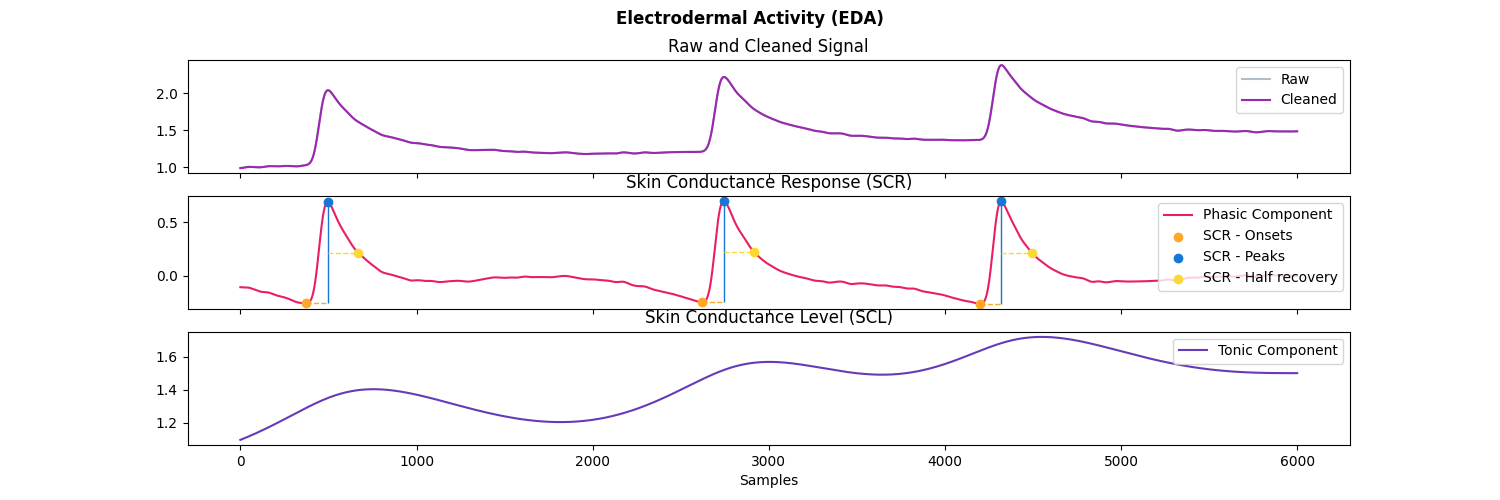
\includegraphics[width=\textwidth]{./images/eda-simulation.png}
    \caption{Decomposition of Raw EDA signal in its two components}
    \label{fig:eda-example}
\end{figure}

The raw signals were generated thorugh NeuroKit2, a Python Toolbox for Neurophysiological Signal Processing that implements several biosignal processing routines, including EDA-related ones \cite{neurokit}.

\subsection{Use Cases}\label{subsec:eda-usecases}

The application of psychophysiological sensors is becoming an increasingly frequent practice in the context of Human Computer Interaction \cite{eda-hci}. More specifically, the Electrodermal Activity may provide a measure to define the level of \textbf{arousal} that characterizes and individual during experimentations and, generally, the usage of specific technologies.

Recent studies involved, for example, the measurement of Heart Rate and Electrodermal Activity in order to define an objective evaluation method for experiences based on \textbf{virtual reality}. Moreover, excellent results have been obtained by Sánchez-Reolid \textit{et al., 2018}~\cite{edasvm}, whose classification model based on \textbf{Deep Support Vector Machines} achieved excellent results in the identification of stress patterns by employing EDA measurements acquired from a wearable device.

\section{Electrodermal Activity and Fall Detection Systems}\label{sec:eda-fall-detection}

The Electrodermal Activity measurement in the context of fall detection has not been a true object of interest yet. It is, however, reasonable to assume that analyzing the skin conductance response may help to provide additional information in order to help classifiers to reach higher levels of accuracy. 

In 2013, T. Horta \textit{et al., 2018}~\cite{eda-fall-detection} included EDA signals in the development of a system for fall detection and prevention based on biofeedback monitoring solutions. The latter obtained valid results, but the analysis performed by the authors did not aim to provide assessments on the influence that Electrodermal Activity had on the accuracy of the whole system (which include other bio-sensors such as electroencephalography, electrocardiogram, electromyography and blood volume pressure).

\subsection{Correlations between EDA and Wearable Devices}\label{subsec:eda-wearables}

Because of the nature of EDA signals, during the years the main object of interest has been monitoring patients over extended periods of time and in real-life situations in order to identify patterns that are difficult to replicate in artificial environments. This has consequently focused the interest of researchers in the development of wearable devices for the electrodermal activity measurement \cite{poh-wearable}. 

In 2010, Poh \textit{et al., 2018}~\cite{poh-wearable} described one of the first implementations of a compact and cost-effective wearable sensor for unobtrusive and long-term assessment of Electrodermal Activity. This was packed inside a wristband exposing two electrodes. The outcomes obtained were strongly correlated with FDA-approved measurement systems. Furthermore, over the last decade several companies such \textbf{Empatica} (an MIT spin-off) or \textbf{Movisens GmbH} (a global leader in ambulatory assessment solutions) implemented highly performing wearable devices for EDA measurement which have been commonly employed in the field of research.

Additionally, at the end of September 2020 \textbf{Fitbit} released \textbf{Sense}, the first commercial wearable device implementing EDA measurement as one of its key features \cite{fitbit-eda}. This opened the way to new opportunities for developers, that will ghopefully be able to build software in order to measure and analyse the Electrodermal Activity by employing Application Programming Interfaces of commercial and commonly diffused devices, without having to rely on expensive and invasive equipment.
% Useful? 

% https://www.ncbi.nlm.nih.gov/pmc/articles/PMC2892750/#:~:text=Electrodermal%20activity%20(EDA)%20refers%20to,et%20al.%2C%201981).


